\chapter{Method}
    Our idea was to apply the method from \citetitle{luo2020consistent}~\cite{luo2020consistent} to fine-tune a CNN and use the refined depth estimates, as well as the inherently produced COLMAP camera in- and extrinsics for 3D reconstructions.
    Before reconstructing, we wanted to improve the initial pose estimates from COLMAP with an energy minimization approach in the fashion of \citetitle{dai2017bundlefusion}~\cite{dai2017bundlefusion}.

    \section{Depth Estimation}
        The geometric loss proposed in \citetitle{luo2020consistent} already requires a lot of geometric information of the scene, which is also required for 3D reconstruction.
        Luo et al. use COLMAP to extract SIFT points from every frame of the input video and then match these points exhaustively to calculate precise camera parameters for the entire scene.
        They then create accurate masks of optical flow between two frames through forward-backward consistency check of FlowNet estimates.
        If enough pixels are valid, a pair of frames is used for training.
        During training, they project the depth estimates of one frame to the coordinate frame of the other image and compare it with the values of that prediction at the positions given through the optical flow masks.
        The loss is comprised of two parts, spatial and disparity loss.
        The spatial loss is the difference between the target pixel position through projection and the position from FlowNet.
        The disparity loss gives the absolute distance between the z-components of the two depth vectors in a common 3D camera space.
        They combine these losses and backpropagate them through the depth estimation network.
        Since the camera in- and extrinsics, as well as the flow masks, are fixed for the fine-tuning, the only way for the model to reduce this error is to produce depth maps which result in basically unique points in the common global coordinate frame for this input.
        They use every consecutive frame pair for training, resulting in temporal consistency, but also more distant pairs in a hierarchical manner, for higher geometric consistency.\\
        To make the depth maps of the CNN comparable to the extrinsics produced by COLMAP, they have to calibrate the relative scale.
        In order to do this, they let COLMAP produce semi-dense depth estimates from the sparse reconstruction results and compute the difference in ratio to the CNN for every frame.
        They then simply divide the camera translations by the mean of the scales to bring the extrinsics into the range of the initial CNN depth maps.\\
        This brings us to our first problem with the realization of the consistent depth maps.
        For the calibration of the scale, they invert the semi-dense COLMAP depth map by simply doing $inv\_cmp\_dpt = 1 / cmp\_dpt$ in their code.
        During execution, this lead to cases where we encountered division by zero in the scale calibration.
        We believe that this made the training unstable, since we had the issue that the loss of the network sometimes became NaN during an epoch.
        We tried to fix this by adding a small $eps$ to the COLMAP depth maps and afterwards we did not encounter NaNs or division by zero anymore.\\
        We don't want to blame the issues entirely on this, since we did not do enough testing to rule out other possibilities, especially since this did not fix our second issue with the consistent depth maps, namely holes in the predicted depth map at random locations (but consistent for the sequence).
        \begin{figure}
            \centering
            
\includegraphics[width=0.33\textwidth]{images/hole.png}
            
\includegraphics[width=0.33\textwidth]{images/hole_zoom.png}
            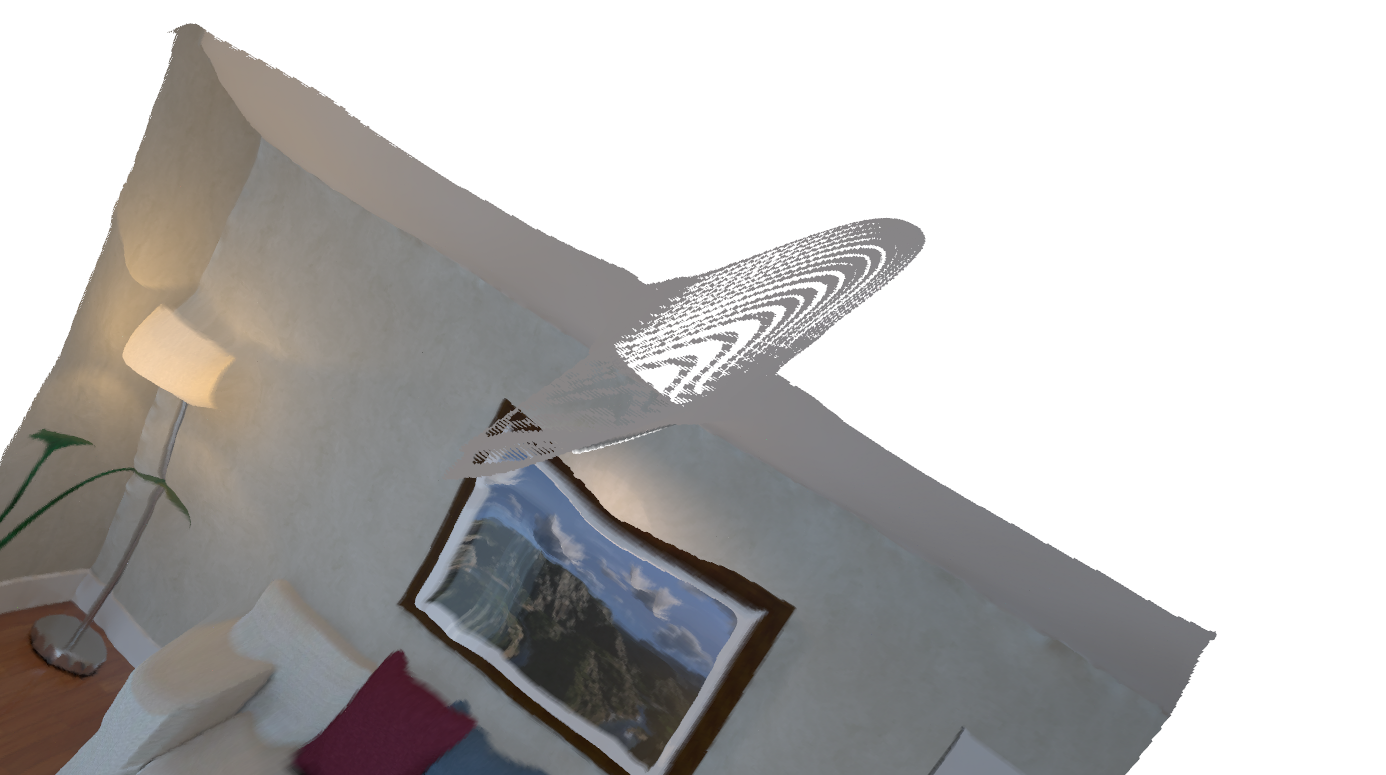
\includegraphics[width=0.33\textwidth]{images/hole_recon.png}
            \caption{Hole in the top corner of the image with basically infinite depth leads to huge deformations of the 3D reconstruction.}
            \label{holes}
        \end{figure}
        Figure~\ref{holes} shows an example of such a black hole present in the predictions for the ground truth dataset.
        These holes add a massive error to the reconstruction, influencing the scaling of the image and making consistent volume integration at these locations impossible.
        We have no idea what causes this problem and how we should counter it, leaving the depth maps from this approach flawed.
        We still use these results as well as the sparsely optimized COLMAP parameters for further optimization.
    
    \section{Pose Optimization}\label{sec:method_pose_optimization}
        Using the estimates for the depth and global pose from the previous step, we technically have everything we need for a 3D reconstruction.
        Before that we wanted to improve on the pose estimation by closely following the methods employed in \citetitle{dai2017bundlefusion}~\cite{dai2017bundlefusion}.
        The hierarchical structure they propose is required for their online reconstruction as it drastically reduces the computational requirements.
        As we aimed for an offline reconstruction, we were able to cut a few of the optimization steps they employed.\\
        Their method for the pose optimization contains a sparse part and a dense part.
        As the reconstruction progresses they reduce the weight of the sparse term and increase the weight of the dense term.
        Since we start with the sparse pose estimation from COLMAP and want to simply refine our poses, we ignore their sparse term and focus on the dense term.\\
        The optimization we implemented is formulated as an error minimization problem where the total dense error is the sum of the photometric and geometric error:
        \begin{equation}
            E_{\text{dense}}(X) = E_{\text{photo}}(X) + E_{\text{geo}}(X)
            \label{eq:edense}
        \end{equation}
        Where $X$ contains the global pose $T$ of every image.
        Both Terms are evaluated over all valid image pairs.
        Two images are considered a valid image pair, if two conditions are met.
        The camera angle difference between two frames has to be below a threshold that we ended up setting to 50\textdegree.
        The second requirement for an image pair is a minimum overlap of 20\%.
        We precompute the image pairs and store them in a matrix $M$ of size $N \times N$ with $M(i,j) = 1$ if $i$ and $j$ form a valid image pair.\\
        The photometric term is based on the luminance gradient $I$, as it is more robust against lighting changes.
        \begin{equation}
            E_{\text{photo}}(X) =
            \frac{1}{v} \sum_{(i,j) | M(i,j)=1}\sum_{k=0}^{\left\lvert I_i \right\rvert}
            \left\lvert\left\lvert
            I_i(K(d_{i,k})) - I_j(K(T_j^{-1}T_id_{i,k}))
            \right\rvert\right\rvert_2^2
            \label{eq:ephoto}
        \end{equation}
        Where $K$ are the camera intrinsics, $d_{i,k}$ is the 3D position of the pixel $k$ in image $i$, and $v$ is the number of valid pixels that contributed to the error.
        A pixel is considered valid if it's 3D position lies within the view frustum of the other camera position.
        \begin{equation}
            E_{\text{geo}}(X) =
            \frac{1}{v} \sum_{(i,j) | M(i,j)=1}\sum_{k=0}^{\left\lvert D_i \right\rvert}
            \left[
            n_{i,k}^T \left(d_{i,k} - T_i^{-1}T_jK^{-1} \left( D_j \left( K\left( T_j^{-1}T_id_{i,k} \right) \right) \right)\right)
            \right]^2
            \label{eq:egeo}
        \end{equation}
        While $I_i(x,y)$ gives us the luminance gradient at an image coordinate $(x,y)$ within image $i$, $D_i(x,y)$ provides us with the depth at the specified pixel in image $i$.
        $n_{i,k}$ is the normal vector at pixel $k$ in image $i$, we compute the normals with open3d.\\
        We believe some further elaboration regarding equations~\ref{eq:ephoto} and \ref{eq:egeo} may be useful.
        For one, the left part of equation~\ref{eq:ephoto},
        \begin{equation*}
            I_i(K(d_{i,k})),
        \end{equation*}
        is simply the luminance at pixel $k$ in image $i$.
        While $K^{-1}(d_{i,k})$ results in a 3D vector, the last dimension can be removed in order to obtain the pixel coordinates $x$ and $y$.
        Then $I_i(x,y)$ is essentially a function that maps the pixel coordinates to the 2d luminance gradient vector.
        For the right side of equation~\ref{eq:ephoto},
        \begin{equation*}
            I_j(K(T_j^{-1}T_id_{i,k})),
        \end{equation*}
        we have to consider that $d_{i,k}$ is a 3D vector and the transforms $T_i$ and $T_j^{-1}$ are both $4 \times 4$ matrices.
        Therefore $d_{i,k}$ has to be expanded by one dimension by appending $1$ to it.
        It can then be transformed by $T_i$ and $T_j^{-1}$.
        The resulting 4D vector has to be reduced to a 3D vector before the inverse intrinsics can be applied to it in order to obtain the pixel coordinate.\\
        For the purpose of understanding these terms we have visualized the following equation for an image pair $(i, j)$:
        \begin{equation}
            C_j(K^{-1}(T_j^{-1}T_id_{i,k})) \coloneqq C_i(K^{-1}d_{i,k})
            \label{eq:vis_perspective}
        \end{equation}
        The visualization of equation~\ref{eq:vis_perspective} can be seen in figure~\ref{fig:vis_perspective}.
        The combination of $T_j^{-1}T_i$ transforms the 3D point $d_{i,k}$ of image $i$ into the global pose of image $i$ and then out of the pose of image $j$.
        The combination is then simply the transform from image $i$ to image $j$.
        In other words, we look at the 3D point $d_{i,k}$ from the camera position of image $j$.
        With the inverse of the intrinsics matrix we retrieve the pixel coordinates that this point would fall into if viewed from the new position.
        For the visualization we write the color information of every pixel from image $i$ into the new pixel position in image $j$.
        All pixels in image $j$ that haven't been hit are set to zero.
        \begin{figure}[ht]
            \centering
            \begin{subfigure}[b]{.45\textwidth}
                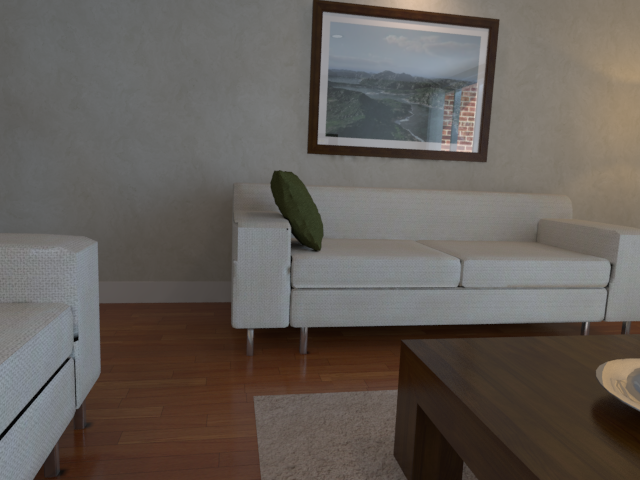
\includegraphics[width=.95\textwidth]{images/vis_perspective_01}
                \caption{original image $i$}
                \label{sfig:i_original}
            \end{subfigure}
            \begin{subfigure}[b]{.45\textwidth}
                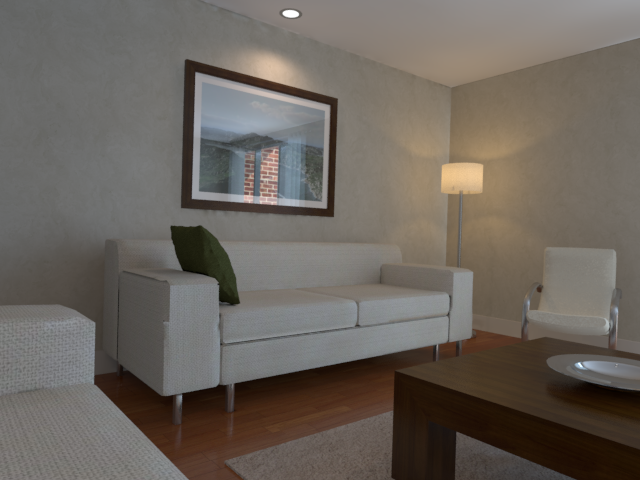
\includegraphics[width=.95\textwidth]{images/vis_perspective_03}
                \caption{original image $j$}
                \label{sfig:j_original}
            \end{subfigure}
            \begin{subfigure}[b]{.45\textwidth}
                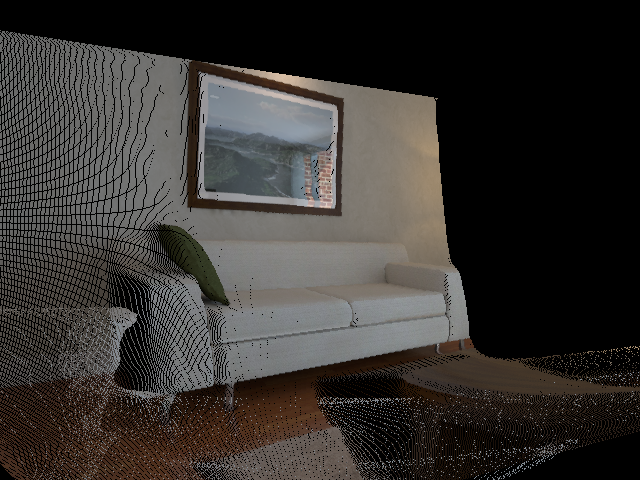
\includegraphics[width=.95\textwidth]{images/vis_perspective_02}
                \caption{information from image $i$ viewed from the camera position of image $j$}
                \label{sfig:i_from_j}
            \end{subfigure}
            \caption[]{Visual interpretation of what happens in the error terms $E_{\text{geo}}$ and $E_{\text{phoyo}}$, described through equation~\ref{eq:vis_perspective}}
            \label{fig:vis_perspective}
        \end{figure}
        In order to solve the minimization problem from equation~\ref{eq:edense} we use the function scipy.optimize.minimize.
        While this is a very inefficient and slow process, it manages to obtain a more fitting set of extrinsics according to our cost function.
        We still took several measures to reduce the computational complexity as much as possible.
        We precompute the initial positions $d_{i,k}$ of each pixel in camera space, since they are identical for each image, before being scaled with the individual depth.
        For each image pair we then just multiply the depth map with each $d_{i,k}$, compute the entire transformation
        \begin{equation}
            T_{ijK} = K(Tj^{-1}Ti),
        \end{equation}
        and finally perform a single vectorized tensor dot product of the transformation with the scaled vectors.
        As our final measure, we convert the $3\times3$ rotation for the optimizer to Euler angles, since this greatly reduces the dimensionality of the problem to be solved, leaving 6 unknowns for each image.
        We multithreaded the energy computation to make use of our 12 core processors.

    \section{3D Reconstruction}
        
        \todo{my reason to skip pose estimation for now is, that it is a bit of a story.\\
        1 get depth \& extrinsics\\
        2 use them\\
        3 improve on extrinsics.\\
        we tried out different approaches for the reconstruction and ended up using open3D\\
        talk about modifying the extrinsics to make everything work\\
        maybe talk about integration and deintegration (used by bundle fusion as it is live and they update their reconstruction)\\
        to improve on the shitty reconstruction we wanted to optimize the extrinsics. this would nicely lead into the next section!!!\\
        compare extrinsics to ground truth with the matlab 3D plot?}